\documentclass{article}

\usepackage[toc]{appendix}
\usepackage[english]{babel}
\usepackage[a4paper,top=2cm,bottom=2cm,left=3cm,right=3cm,marginparwidth=1.75cm]{geometry}
\usepackage{amsmath,amssymb}
\usepackage{graphicx}
\usepackage{xcolor}
\usepackage[colorlinks=true, allcolors=blue]{hyperref}
\usepackage{float} %for å kontrollere bildeplasseringene 
\usepackage{caption}
\usepackage{lipsum}

\renewcommand\thesubsection{\alph{subsection})} %Gjør at subsection blir a) i stedet for 1.1.1
\newcommand{\vect}[1]{\boldsymbol{{#1}}} %en ny kommando som sier at \vect gir fet skrift. det er alternativ vektornotasjon.


\title{Oppgave 1}
\author{Ole Sandok}

\begin{document}
\maketitle

\begin{abstract}
tekst
\end{abstract}

\tableofcontents

\section{ }


\section{}
vi ønsker å løse integrallikningen:
\begin{equation}
    -\pi \phi(\bar{x}\bar{y})  + \int_{S} \phi  \frac{\partial }{\partial n} \ln r dS = \int_{S}  \frac{\partial \phi}{\partial n} \ln r dS
\end{equation}
der $\partial \phi / \partial n = n_1$ langs med S.

Diskret integrallikning.
\begin{equation}
    -\pi \phi  + \Sigma_{m=1}^N \phi_m (-\Delta \Theta_{n,m})   =  \sum_{m=1}^N [\frac{\partial \phi}{\partial n}]_m h_{n,m}
\end{equation}

Addert masse kan approksimeres slik:
\begin{equation}
    m_{ij}  = \rho \int_{S} \phi_j n_i dS \, \simeq \, \rho \sum_{m=1}^N [\phi_j]_m  [n_i]_m \Delta S_m.
\end{equation}





\section{Figurer}
\subsection{Diskretisering av ellipse}





{\noindent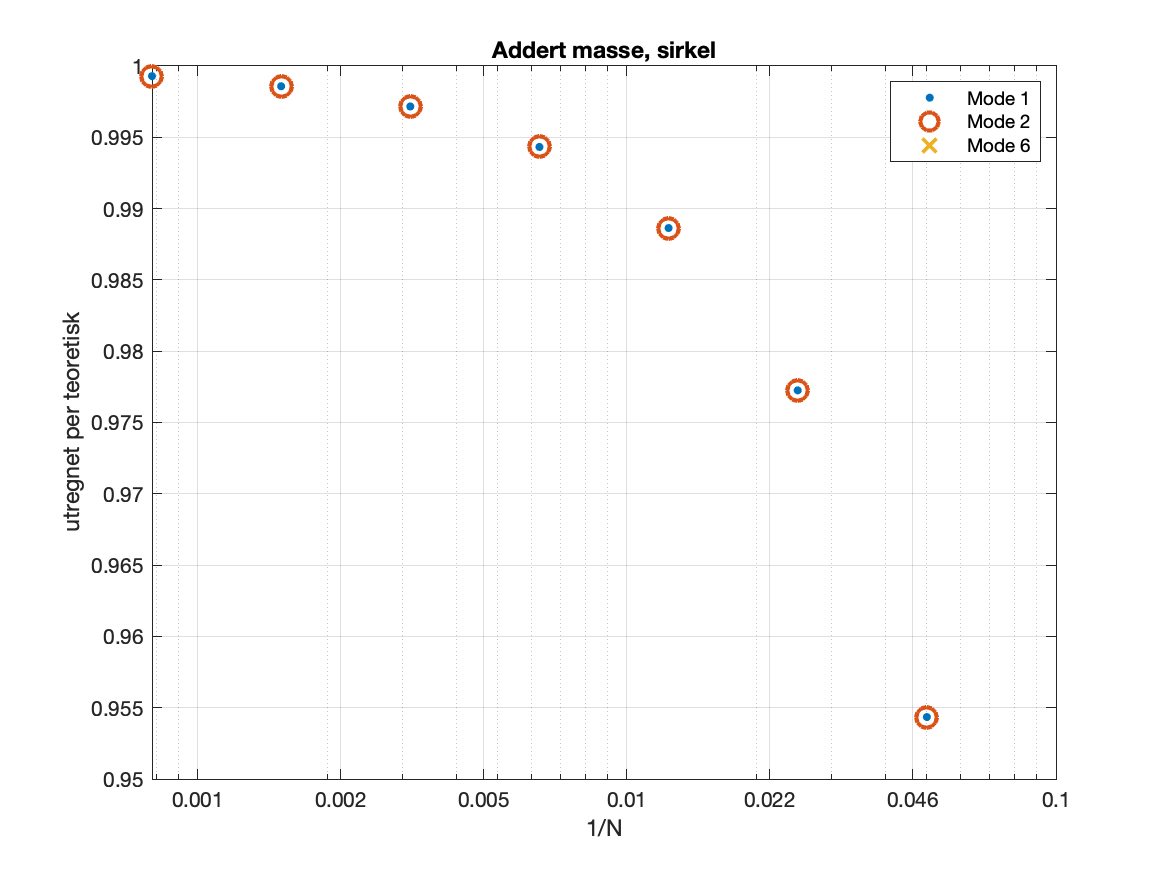
\includegraphics[width=\linewidth]{/Users/ole/Tex/MEK4420/oblig1images/m11_sirkel.png}
\captionof{figure}{}}

{\noindent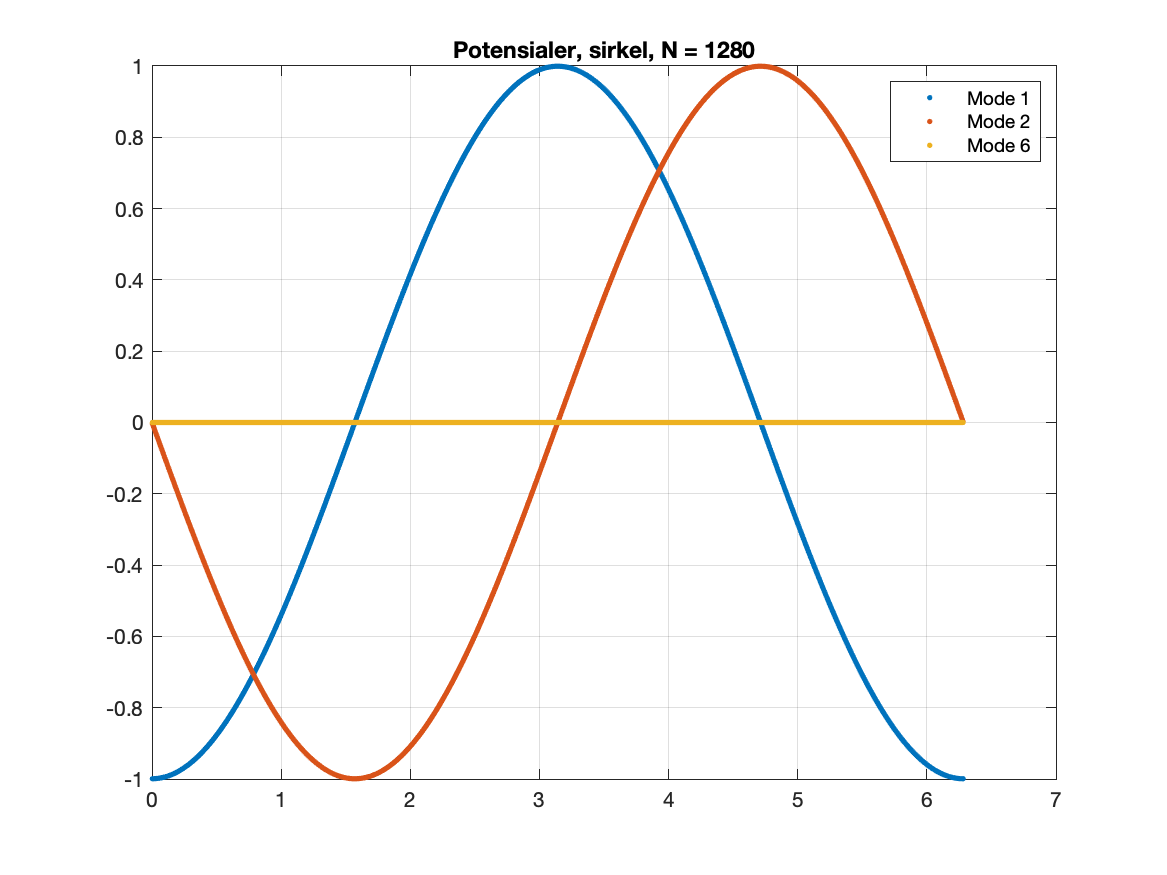
\includegraphics[width=\linewidth]{/Users/ole/Tex/MEK4420/oblig1images/potensialer_sirkel.png}
\captionof{figure}{}}




%--------------------ellipse b/a = 0.1


{\noindent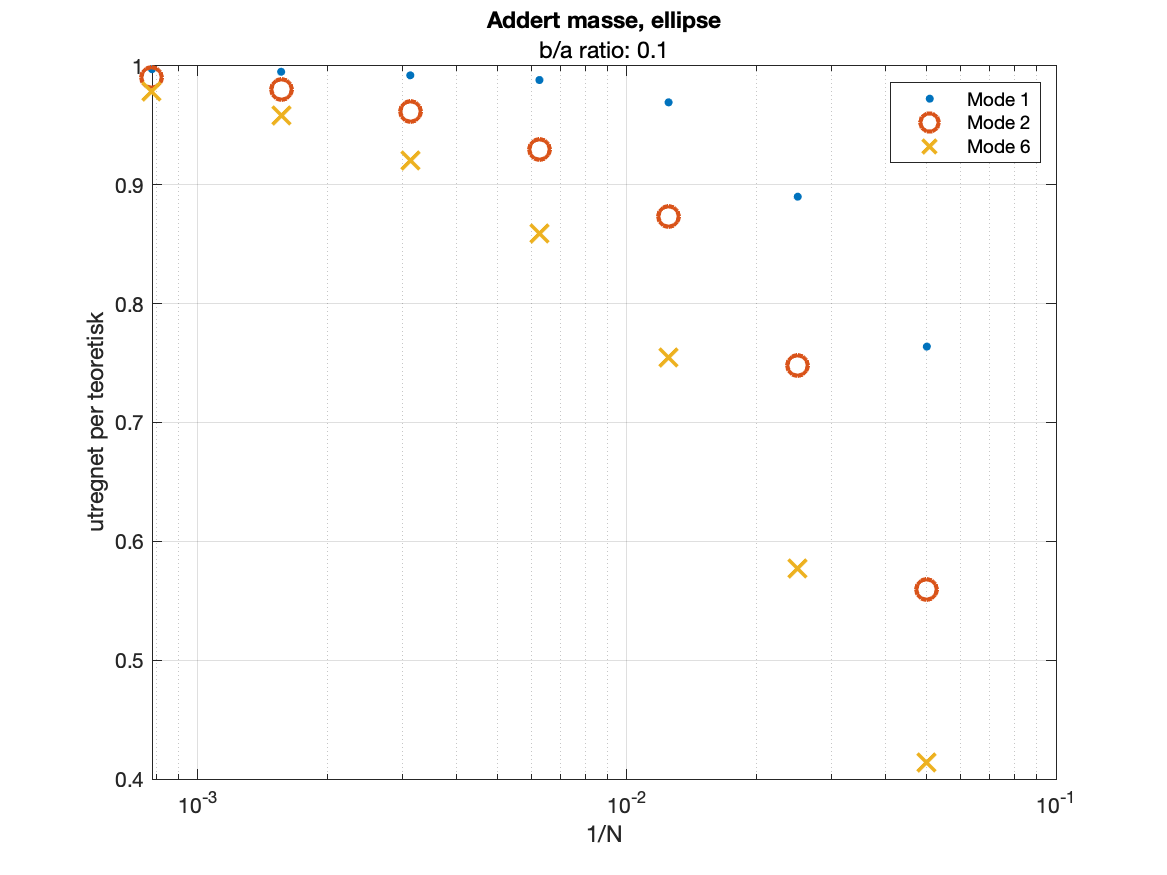
\includegraphics[width=\linewidth]{/Users/ole/Tex/MEK4420/oblig1images/m11_ellipse.png}
\captionof{figure}{}}

{\noindent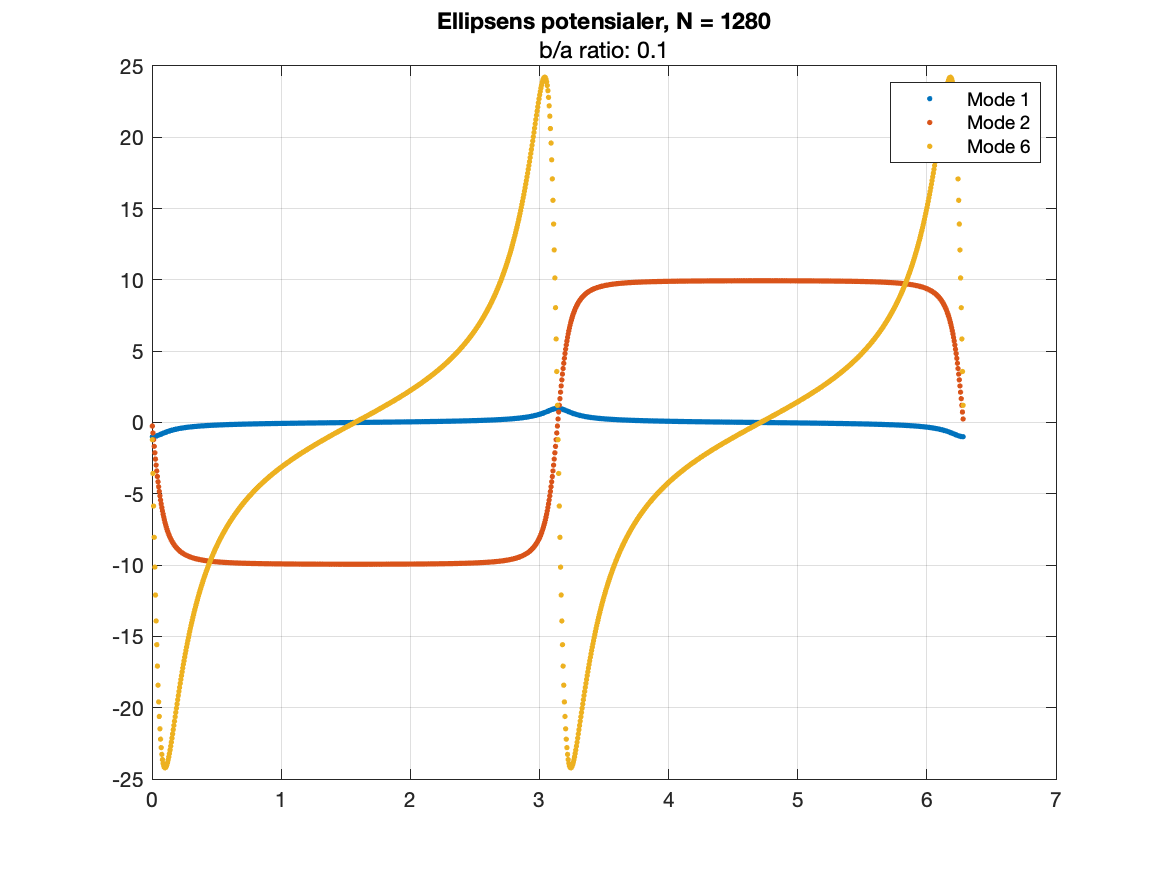
\includegraphics[width=\linewidth]{/Users/ole/Tex/MEK4420/oblig1images/potensialer_ellipse.png}
\captionof{figure}{}}


%--------------------ellipse b/a = 0.5

{\noindent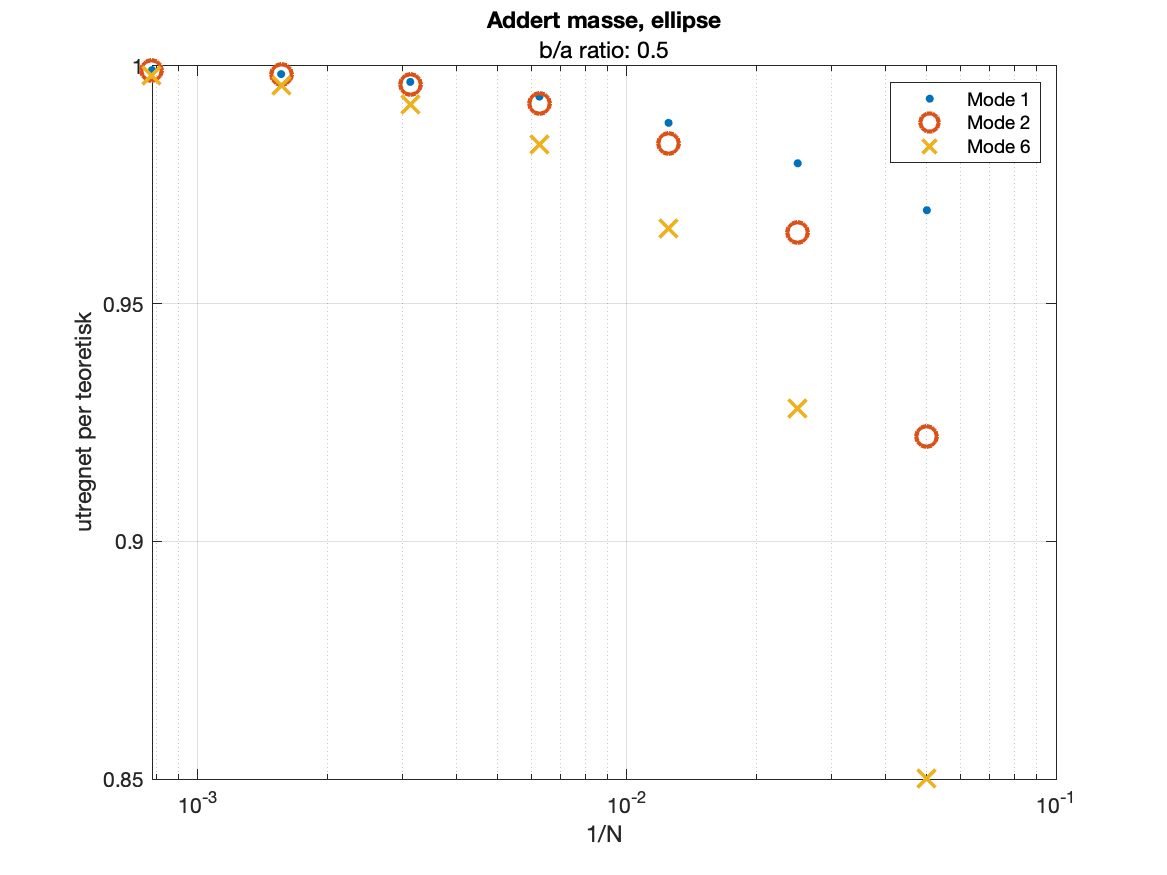
\includegraphics[width=\linewidth]{/Users/ole/Tex/MEK4420/oblig1images/m11_2ellipse.png}
\captionof{figure}{}}

{\noindent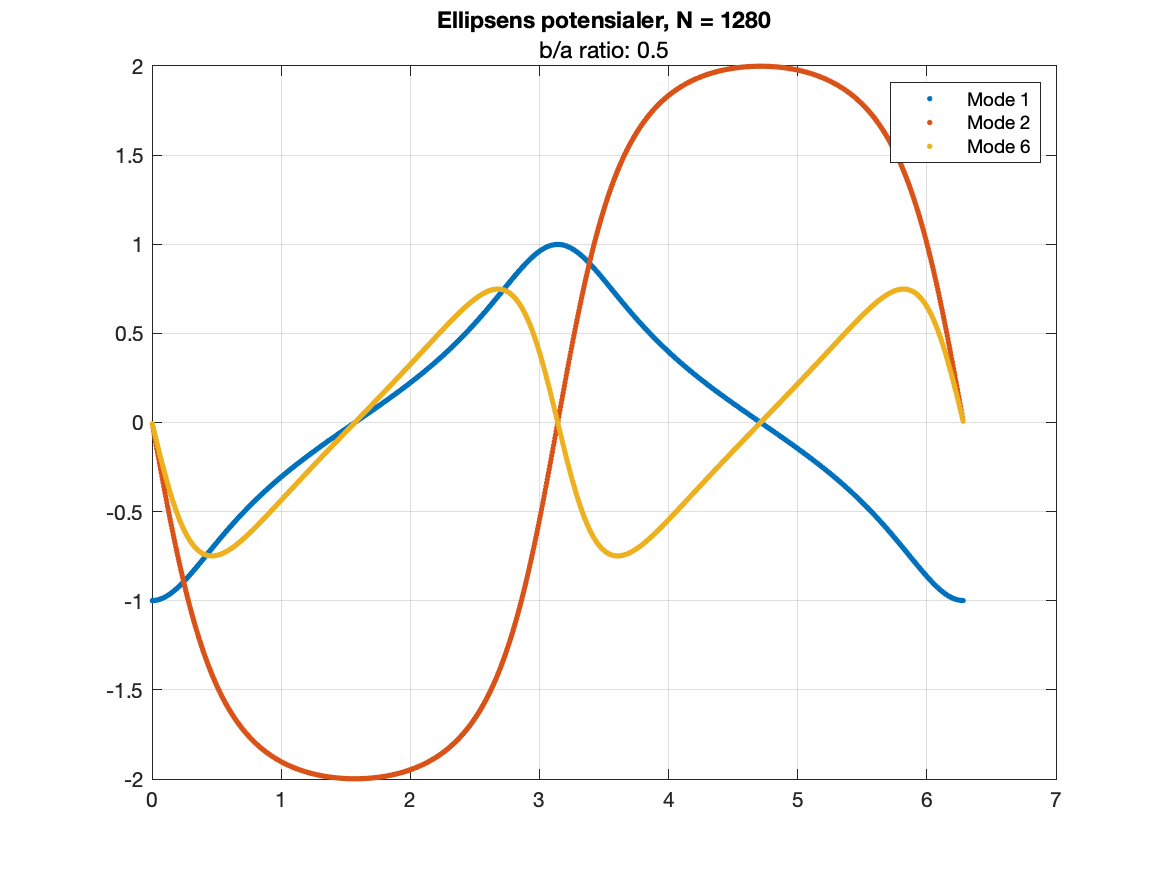
\includegraphics[width=\linewidth]{/Users/ole/Tex/MEK4420/oblig1images/potensialer_2ellipse.png}
\captionof{figure}{}}


%--------------------diskretisering ellipse
{\noindent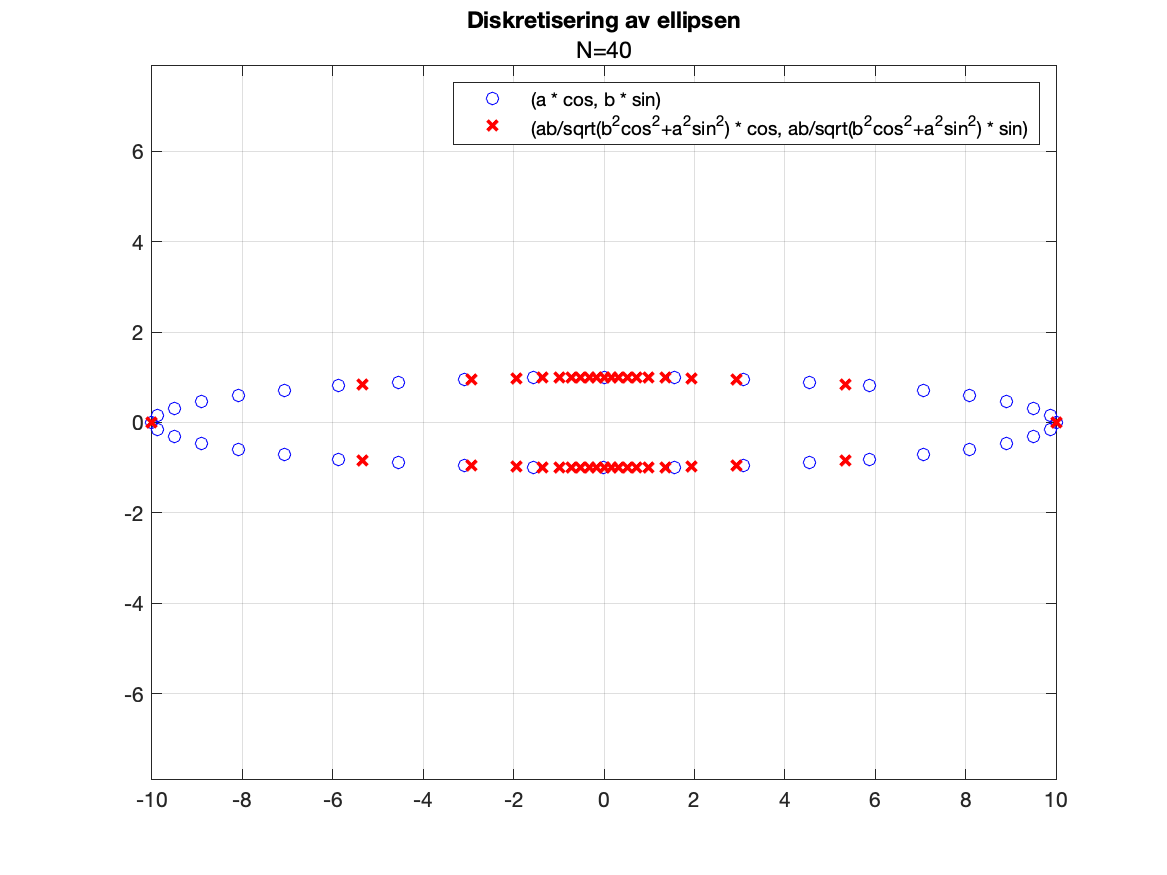
\includegraphics[width=\linewidth]{/Users/ole/Tex/MEK4420/oblig1images/diskretisering_ellipse.png}
\captionof{figure}{de røde kryssene er fordelingen som er brukt. De blå sirklene er "normal" fordeling}}

{\noindent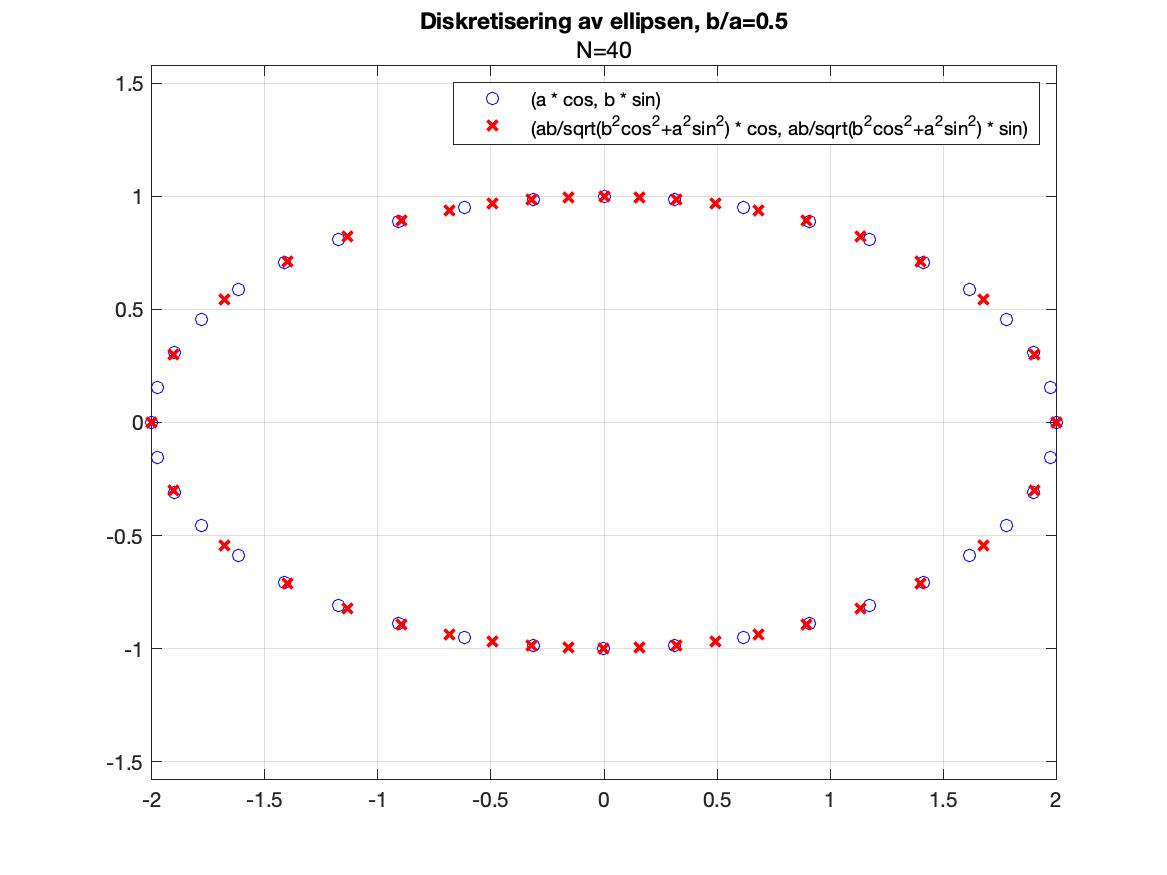
\includegraphics[width=\linewidth]{/Users/ole/Tex/MEK4420/oblig1images/diskretisering_2ellipse.png}
\captionof{figure}{}}


%--------------------kvadrat
\section{Kvadrat}

{\noindent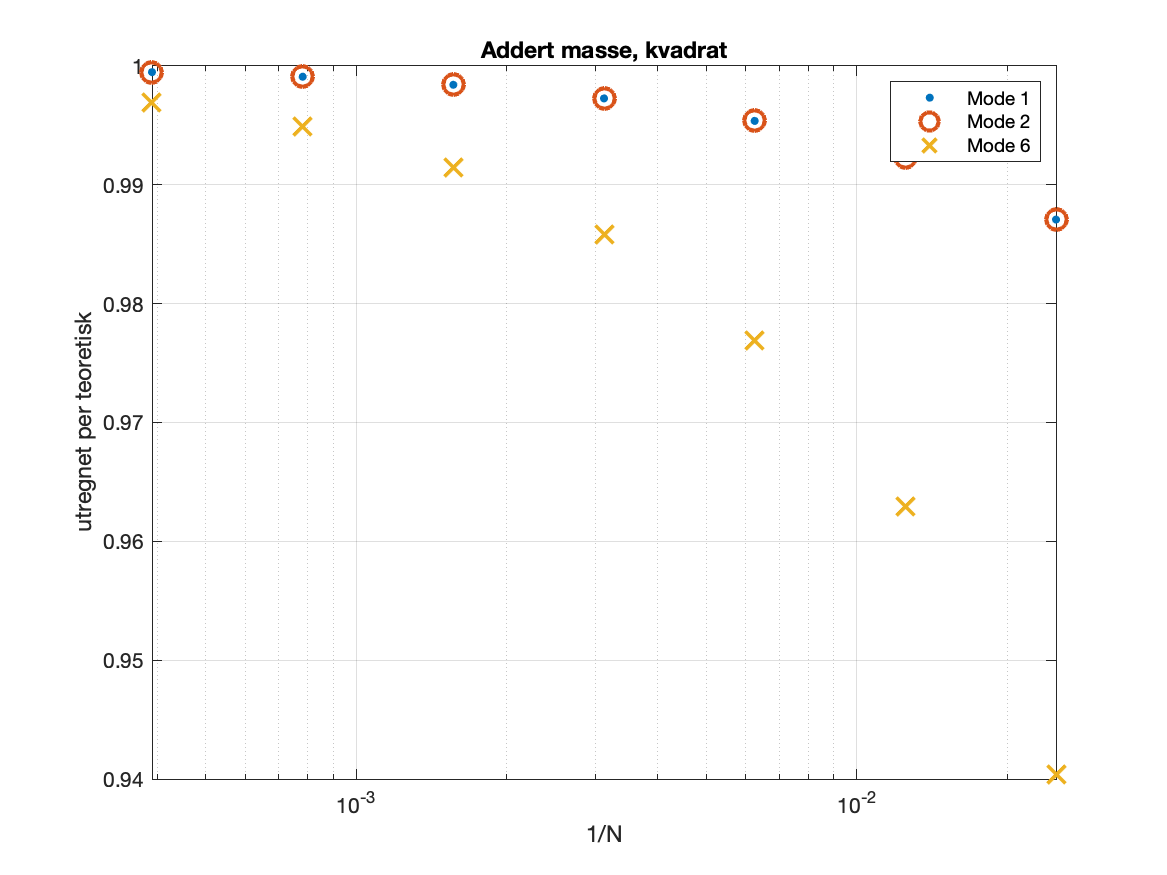
\includegraphics[width=\linewidth]{/Users/ole/Tex/MEK4420/oblig1images/m11_kvadrat.png}
\captionof{figure}{}}

{\noindent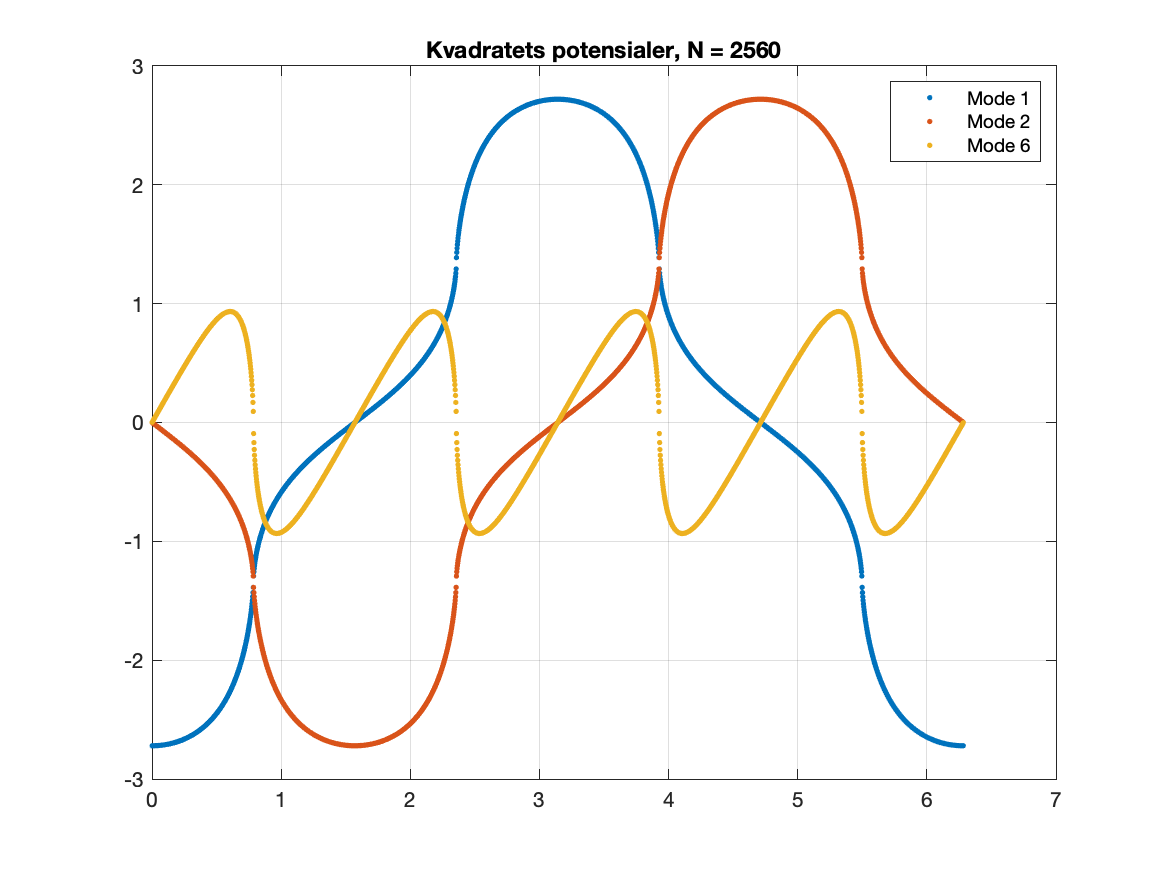
\includegraphics[width=\linewidth]{/Users/ole/Tex/MEK4420/oblig1images/potensialer_kvadrat.png}
\captionof{figure}{}}
\end{document}

